\subsection{Salience Biased Affinity Propagation}
\begin{frame}{Salience Biased Affinity Propagation}
    \center

    \begin{itemize}
        \item \textbf{Affinity Propagation Clustering} 
            \begin{itemize}
                \item Exemplars (and clusters) determined by similarity. 
            \end{itemize}
            ~\\
        \item<2> \textbf{Salience-biased Affinity Propagation Clustering}
            \begin{itemize}
                \item Exemplars likely to have higher predicted salience $\hat{y} \sim p(\cdot|s, q)$ 
            \end{itemize}
    \end{itemize}
   % \only<1>{ \includegraphics[scale=.8]{images/cluster_anim1.pdf} }
   % \only<2>{ \includegraphics[scale=.8]{images/cluster_anim2.pdf} }
   % \only<3>{ \includegraphics[scale=.8]{images/cluster_anim3.pdf} }
    \only<1>{ \includegraphics[scale=.7]{images/cluster_anim4.pdf} }
    %\only<5>{ \includegraphics[scale=.8]{images/cluster_anim5.pdf} }
    %\only<6>{ \includegraphics[scale=.8]{images/cluster_anim6.pdf} }
    \only<2>{ \includegraphics[scale=.7]{images/cluster_anim7.pdf} }



\end{frame}

\begin{frame}
    \frametitle{Experiments}
    
    \begin{itemize}
    \item Leave-One-Out evaluation
        \begin{itemize}
            \item 21 TREC 2014 Temporal Summarization events
        \end{itemize}
        ~\\
        \item 3 events held out for tuning similarity threshold parameters
            ~\\
            ~\\
        \item trained salience models for each event
        \begin{itemize}
            \item 1000 sentences sampled for each event
            \item At test time, salience prediction is the average of the 
                20 other models
        \end{itemize}
    \end{itemize}
    
\end{frame}


\begin{frame}
    \frametitle{Evaluation Metrics}
    \begin{itemize}
        \item \textsc{Rouge}
        \begin{itemize}
            \item ``reference'' summary generated by concatenating event 
                    nugget texts
        \end{itemize}
~\\
    \item TREC Temporal Summarization metrics
        \begin{itemize}
            \item  \textbf{Expected Gain} --- the average number of novel nuggets in 
                each extracted sentence; $\approx$ nugget precision. ~\\~\\
            \item \textbf{Comprehensiveness} --- nugget recall.
        \end{itemize}
%    \item Expected Gain and Comprehensiveness
%        $$\mathbb{E}[\mathrm{Gain}] = \frac{|S_n|}{|S|}\;\;\;\;\;\;\;\;\;
%            \textrm{Comprehensiveness} = \frac{|S_n|}{|N|}$$
%            where \begin{itemize}
%            \item[] $S$ is the set of system updates
%                \item[] $S_n$ is the set of nuggets mapped to updates in $S$
%                \item[] $N$ is the set of nuggets for the event
%            \end{itemize}
    \end{itemize}
\end{frame}

\begin{frame}
    \frametitle{Baselines}
    \begin{itemize}
    \item SAP -- full model: salience-biased affinity propagation
    \item AP -- affinity propagation clustering with no salience
    \item HAC -- hierarchical agglomerative clustering
    \item RS -- rank by salience
    \end{itemize}
\end{frame}

\begin{frame}
    \frametitle{\textsc{Rouge}}
\begin{table}[h]
\centering
% centering table
\begin{tabular}{l c c c}
% creating 10 columns
    \multicolumn{4}{c}{\textsc{Rouge}-$1$}\\
\hline
\hline
% inserting double-line
$\mathrm{System}$ & $\mathrm{Recall}$ & $\mathrm{Prec.}$ & $\mathrm{F}_1$\\
[0.5ex]
\hline
SAP & $\mathbf{0.282}$ & $\mathbf{0.344}$ & $\mathbf{0.306}$\\
AP          & $0.245$ & $0.285$ & $0.263$ \\
RS          & $0.230$ & $0.271$ & $0.247$ \\
HAC         & $0.169$ & $0.230$ & $0.186$ \\
\hline % inserts single-line
\end{tabular}
~\\[1ex]
~\\
\begin{tabular}{l c c c}
% creating 10 columns
    \multicolumn{4}{c}{\textsc{Rouge}-$2$}\\
\hline
\hline
% inserting double-line
$\mathrm{System}$ & $\mathrm{Recall}$ & $\mathrm{Prec.}$ & $\mathrm{F}_1$\\[0.5ex]
\hline
\textsc{SAP} & $\mathbf{0.045}$ & $\mathbf{0.056}$ & $\mathbf{0.049}$\\
\textsc{AP}          & $0.033$ & $0.038$ & $0.035$ \\
\textsc{RS}          & $0.031$ & $0.037$ & $0.034$ \\
\textsc{HAC}         & $0.017$ & $0.024$ & $0.019$ \\
\hline % inserts single-line
\end{tabular}
\end{table}
\end{frame}


\begin{frame}
    \frametitle{\textsc{Rouge}-1 over time}
\begin{center}
\includegraphics[]{images/rouge-time.eps}
\end{center}
\end{frame}


\begin{frame}
\frametitle{$\mathbb{E}[\mathrm{Gain}]$ and $\mathrm{Comprehensiveness}$}
\begin{center}
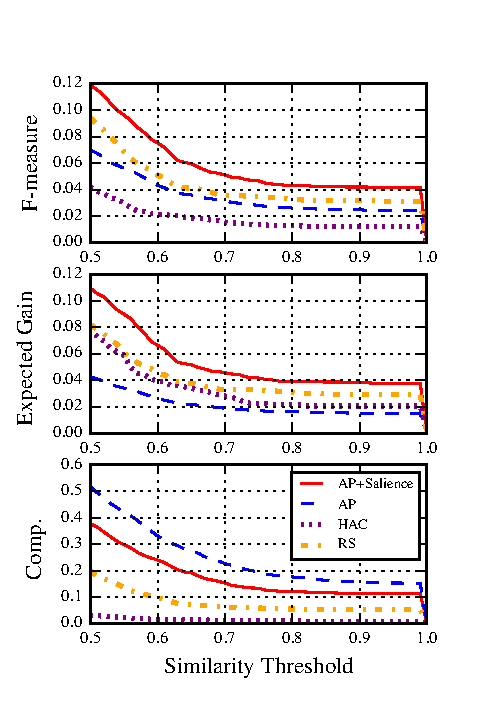
\includegraphics[scale=.7]{images/nuggets-metrics2.eps}
\end{center}
\end{frame}


